\documentclass[12pt, letterpaper]{article}
\usepackage[utf8]{inputenc}
\usepackage{sectsty}
\usepackage{graphicx}
\usepackage{hyperref}
\usepackage[labelfont=bf]{caption}
\usepackage{nopageno}
\usepackage{subcaption}
\captionsetup{compatibility=false}

\sectionfont{\fontsize{16}{15}\selectfont}
\subsectionfont{\fontsize{14}{15}\selectfont}

\title{Catboost Classifiers for LHCb Decay Triggering}
\author{Sean Condon\thanks{scondon@mit.edu}}
\date{June 2020}

\begin{document}

\maketitle

\section{Introduction}

The Large Hadron Collider beauty (LHCb) experiment requires a series of high level triggering (HLT) algorithms to reduce its enormous data output rate of roughly 40 Tbit/s down to a more manageable data stream that can be stored and analyzed offline. As LHCb prepares for its third data collection run, the previously used triggering algorithms need to be reoptimized for run 3 data taking conditions. In the document, I explore the use of the Catboost Library\footnote{\url{https://catboost.ai/}} to produce boosted decision trees capable of classifying LHCb noise versus signal with acceptable efficiency and false positive rate. 

\section{1-Track \& 2-Track Triggers - June 10th}

\subsection{Methods}

The 1-track and 2-track boosted decision tree classifiers were made with the same input parameters presented in \textit{LHCb Topological Trigger Reoptimization} \footnote{\url{https://arxiv.org/pdf/1510.00572.pdf}}. These parameters are summarized in the table below:

\begin{center}
\begin{table}
\begin{tabular}{ c|c|c } 

 \textbf{Classifier} & \textbf{Analysis Variables} & \textbf{Variable Names}\\ 
  \hline
  & & \\
 1-Track Model & PT, $\mathrm{IP}_{\chi^2}$ & trk\_PT,\\ 
 & &  trk\_IPCHI2\_OWNPV \\
 & & \\
  \hline
  & & \\
 2-Track Model & sum PT, vertex $\chi^2$, FD $\chi^2$,  & (trk1\_PT + trk2\_PT),   \\ 
 & N (\# tracks with $\mathrm{IP}_{\chi^2}$ $<$ 16) & sv\_ENDVERTEX\_CHI2,\\
 &  & sv\_FDCHI2\_OWNPV,\\
 & & N \\
 \end{tabular}
 \caption{Analysis variables for the 1-track and 2-track classifiers, along with their lookup names in the .root files.}
 \end{table}
\end{center}

As of June 10th, no preselections were made on the input data, apart from the $\mathrm{track}_\chi^2 / \mathrm{ndof} < 2.5$ cut that is already applied to the input data. The data used to train the classifiers consists of 6 .root files of different decay modes with some signal and some noise. Each .root file contains 1-track, 2-track, 3-track, and 4-track data. Data from all 6 decay modes was combined to make a generic "interesting decay" trigger. The pooled data is about 92\% noise and 8\% signal, so training examples are weighted by this ratio so that the classifiers train on a balanced dataset. The pooled data was split into 75\% training, and 25\% testing.

The classifiers were CatBoostClassifier models, and all used 'Logloss' as a loss function. To optimize the hyperparameters of the models (iterations - the number of decision trees, depth - the depth of each tree, and learning rate), 96 classifiers were trained each for the 1-track and the 2-track data. Each of these classifiers contained different hyperparamters from the 3D parameter space outlined below:
$$\mathrm{depth} = [6,\:8,\:10,\:12,\:14,\:16]$$
$$\mathrm{learning \: rate} = [0.1,\:0.01,\:0.001,\:0.0001]$$
$$\mathrm{iterations} = [100,\:200,\:400,\:800]$$

After the training process, the performance of all 96 possible hyperparameter configurations was analyzed for both the 1-track and the 2-track models, and this is summarized in the next section.

\subsection{Results}
After being trained, all models were evaluated on the testing dataset and an ROC plot was constructed for each. The evaluation metric used to select the optimal hyperparameters was the integrated ROC curve, a measure of signal detection efficiency (correctly classified signal over total signal) versus false positive rate (noise classified as signal over total noise).

The same hyperparameters had the best performance for both the 1-track and the 2-track classifiers, and the hyperparameters that performed best were:

$$\mathrm{depth} = 8, \: \: \: \mathrm{learning \: rate} = 0.01, \: \: \: \mathrm{iterations} = 800$$

ROC curves for both the 1-track and 2-track models with these hyperparameters are shown in figure \ref{fig:roc1}. It is worth noting that all 96 hyperparameter configurations had an integrated ROC within 5\% of the optimal value, so all configurations had similar performance, and the performance of the boosted decision trees seems quite insensitive to the three hyperparameters examined here, at least within the ranges described above.



\begin{figure}
\begin{center}
\textbf{1-Track Classifier}\\
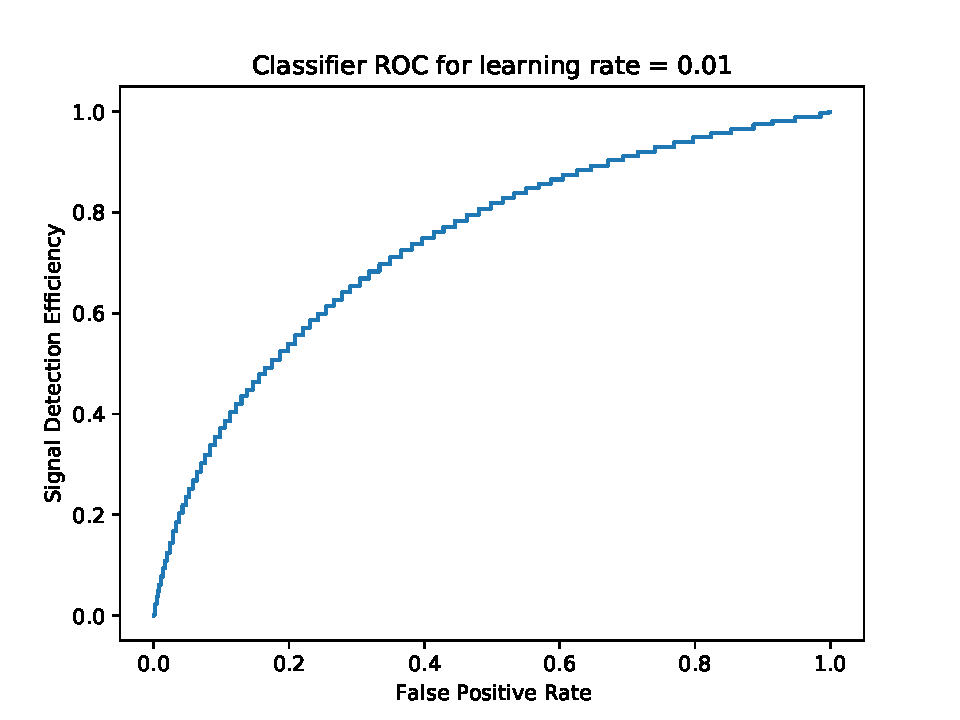
\includegraphics[width=0.87 \textwidth]{oneTrackRoc.pdf}\\
\textbf{2-Track Classifier}\\
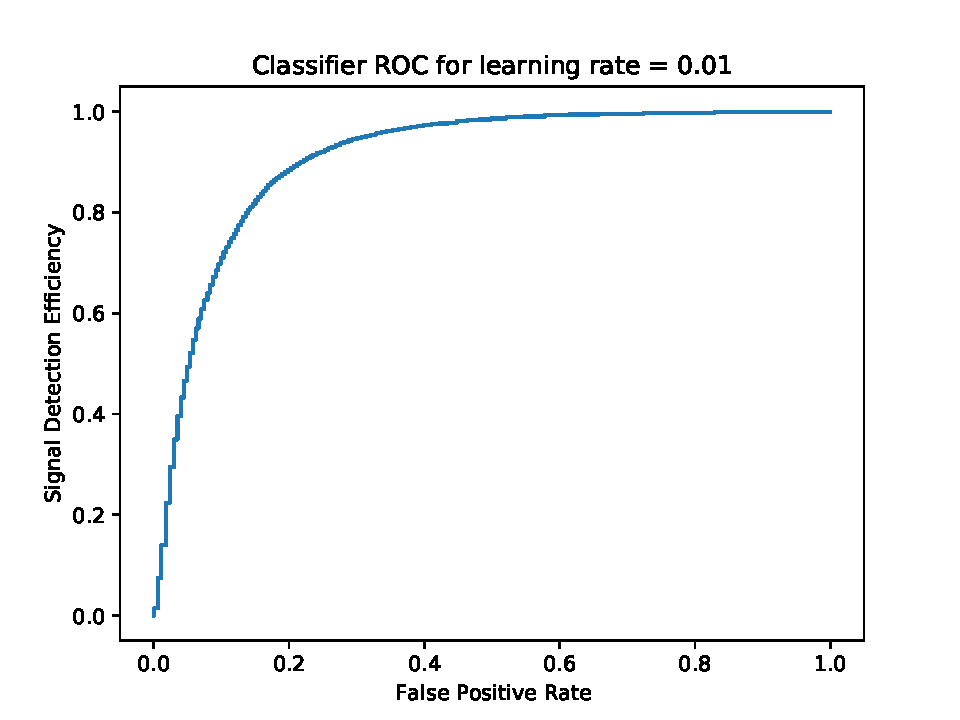
\includegraphics[width=0.87 \textwidth]{twoTrackRoc.pdf}\\
\end{center}

\caption{ROC curves for the optimal 1-track model (above) and the optimal 2-track model (below).}
\label{fig:roc1}
\end{figure}


As expected, the 2-track model performs significantly better than the 1-track model. Using a cutoff of 50\% for the signal probability, we get a 64.16\% signal detection efficiency and a 27.82\% false positive rate for the 1-track model, and a 86.78\% signal detection efficiency and a 18.09\% false positive rate for the 2-track model.

\subsection{Discussion and Next Steps}
Over the next few days I will work on lowering the false positive rate of these detectors, as I'm confident these values are too high for LHCb data taking conditions. I think we can do a couple quick things to greatly improve performance. My ideas on the subject are outlined below, in order of easiest to hardest to implement:
\begin{itemize}

\item Revisit the analysis variables used and make sure these are the correct values to input into the classifier and potentially add new analysis variables to both the 1-track and 2-track classifiers.

\item Examine the decision boundaries between classified noise and signal to see what kinds of noise types the classifiers are routinely mis-identifying.

\item Do more comprehensive preselections to weed out training / testing examples of poorly-fit vertices.

\item Train larger boosted decision trees (more iterations) and then prune these down to less trees while maximizing some criteria (e.g. balanced accuracy) on a validation set that's independent of the training and testing sets.

\item Do hyperparameter optimization on the other classifier hyperparameters besides depth, learning rate, and iterations.

\item Work on implementing a better custom loss function, or try training with the other native loss functions in Catboost.

\end{itemize}


\section{Preselections and Improved ROCs for Triggers - June 17th}

\subsection{Rescaling ROC Plots}
The first improvement that was made on last weeks results was to rescale the ROC plots for each trigger to display their performance more accurately. The first step of this process was simply re-scaling the x-axis of the plots to be an approximate trigger rate of the algorithm. The trigger rate is determined as:

$$\mathrm{Trigger\: rate} = \mathrm{False\:positive\:rate} \:*\: \mathrm{30\: MHz}$$

where 30 MHz is the baseline event rate for run 3 of LHCb. The x-axis of all ROC plots is also displayed logarithmically, so the low end of triggering rates is more clearly visible.

Additionally, we also changed how the triggers process true positive and false positive detections. The one-track and two-track algorithms are applied to each track (or 2-track SV) of a many-track event. Each event in the training data is made up of 3.04 (mean) single tracks for the 1-track data, or 8.18 (mean) 2-track SVs for the 2-track data. A single positively triggered track (or 2-track SV) will trigger the entire event to be sent to the next HLT stage, so we now consider true positive signal detections as any event that is triggered on that contains at least one signal, and a false positive is any event that is triggered on that contains no signal.

%things we've done
%rescaled ROC (discussion of difficulty)
%preselections with results
%overtraining verification (roc comp and also loss during training)
%boundary decision plots
%make a git also

\subsection{Preselections for Improved Performance}
To improve the performance of the algorithms, I also implemented pre-selections to weed out poorly fit vertices from the training and testing data. The preselections used are defined in \footnote{\url{https://arxiv.org/pdf/1510.00572.pdf}}. Table \ref{table:preselect} summarizes the preselections used for the 1-track and 2-track models, along with the amount of data these preselections cut from the training and testing datasets.


\begin{center}
\begin{table}
\begin{tabular}{ c|c|c } 

 Preselection Variable & Preselection & Data cut by selection \\ 
 \hline
 \textbf{1-track Model} &  &  \\ 
 Transverse momentum \& & PT $>$ 500 MeV & 29.12\% \\
 Impact parameter significance & $\mathrm{IP}_{\chi^2} >$ 4 & \\ 
 \hline
 \textbf{2-Track Model} & & \\
 Pseudorapidity ($\eta$) & 2 $< \eta <$ 5 & 10.19\%\\
 Corrected mass (mcor) & mcor $>$ 1 GeV & 0.0\%\\
  Transverse momentum \& & PT $>$ 500 MeV & 49.21\% \\
 Impact parameter significance & $\mathrm{IP}_{\chi^2} >$ 4 & \\ 
 All & & 53.78\% \\
 
 
\end{tabular}
\caption{Preselections made for the 1-track and 2-track models, along with the amount of data those cuts removed.}
\label{table:preselect}
\end{table}
\end{center}

%for 1 track, track cuts = 29.12% tossed
%for 2 track, eta, mcor, eta+mcor+tracks = tossed

\subsection{Results}
Overall, the clustering of tracks into events seems to have decreased performance across the board. I believe this is because the triggers now have more than one chance to trigger on a false positive. For example, because 1-track events are on average made up of ~3 tracks, for noise events the trigger has 3 independent chances to trigger on a noise track, thus we expect an FPR of 3x that of the individual track performance. Because 2-track SV events are made up of on average 8.8 track pairs, the FPR in this algorithm should be even worse compared to its individual track performance.

Regardless, the performance of these new algorithms, with new x-scales, is summarized below. In figure \ref{figure:decayRoc} we see the ROC plots of the best performing pre-selected triggers. The information on preselection performance is more clearly outlined in table \ref{table:preselectPerf}.

\begin{figure}
\begin{center}
\textbf{1-Track Trigger}\\
\end{center}
\begin{minipage}[b]{0.5\textwidth}
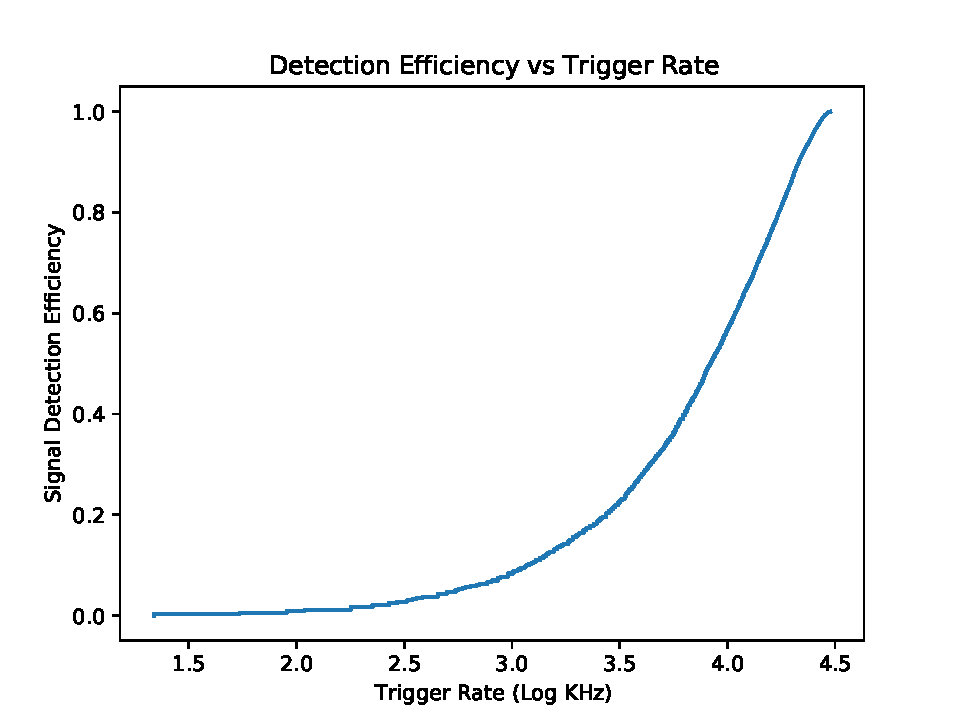
\includegraphics[width=1\textwidth]{1trackRoc.pdf}
\end{minipage}
\begin{minipage}[b]{0.5\textwidth}
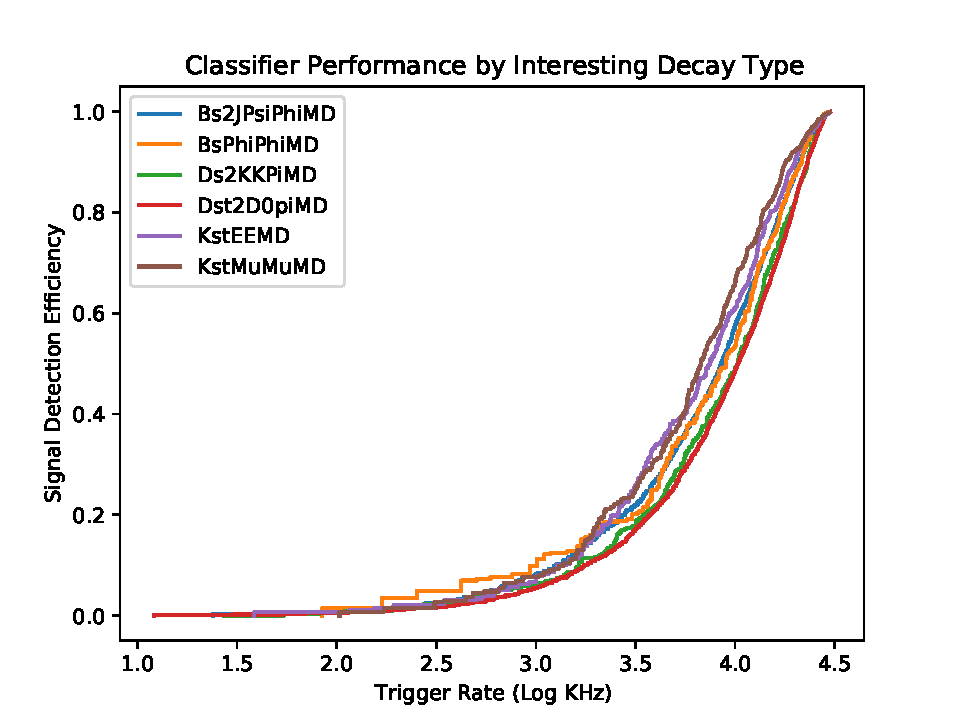
\includegraphics[width=1\textwidth]{1trackDecayRoc.pdf}
\end{minipage}
\begin{center}
\textbf{2-Track Trigger}\\
\end{center}
\begin{minipage}[b]{0.5\textwidth}
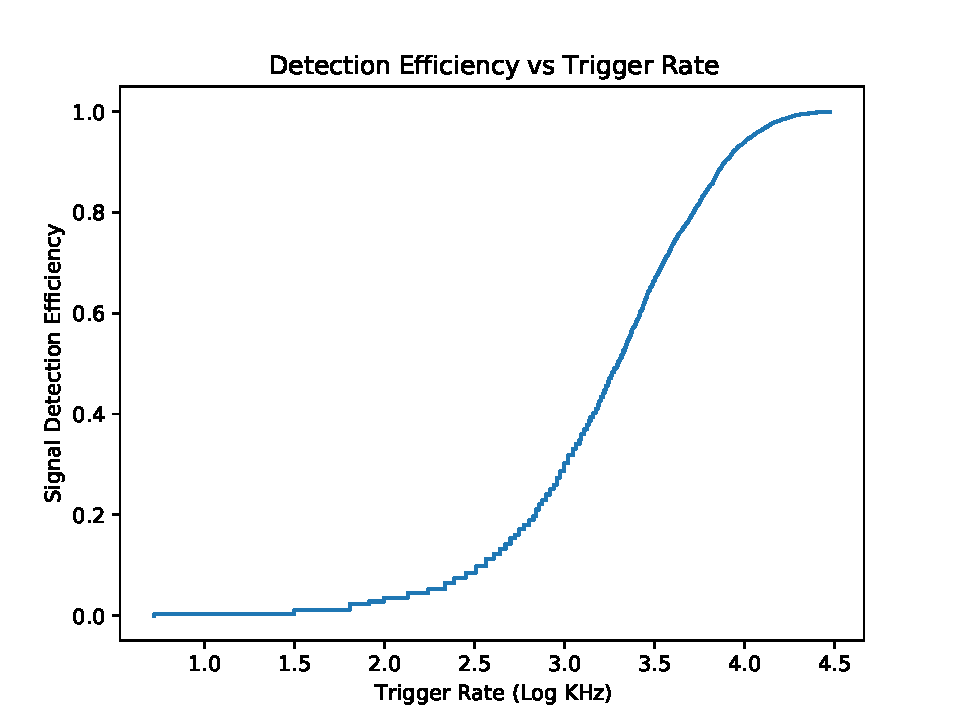
\includegraphics[width=1\textwidth]{2trackRoc.pdf}
\end{minipage}
\begin{minipage}[b]{0.5\textwidth}
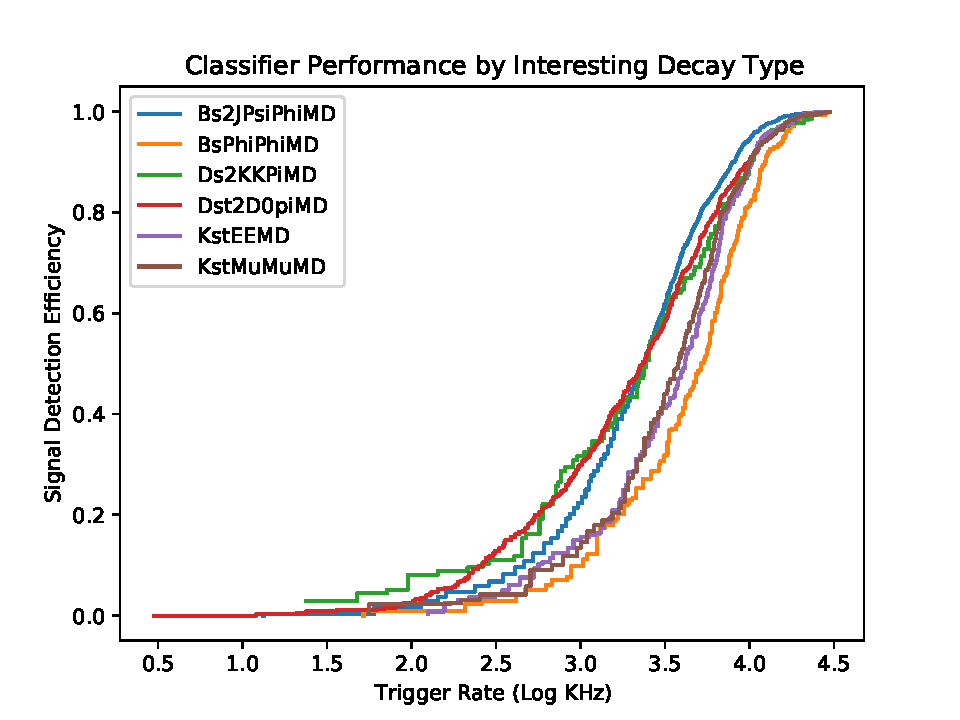
\includegraphics[width=1\textwidth]{2trackDecayRoc.pdf}
\end{minipage}

\caption{Scaled ROC plots for the most effective 1-track and 2-track models. Both are presented with a total ROC and an ROC by signal decay type.}
\label{figure:decayRoc}
\end{figure}




\begin{center}
\begin{table}
\begin{tabular}{ c|c } 

 Preselection Preselection & Performance at Trigger = 1 MHz (efficiency) \\ 
 \hline
 \textbf{1-track Model} &   \\ 
 None &  8.35\%\\
 Transverse momentum \& & 8.79\% \\
 Impact parameter significance &  \\ 
 \hline
 \textbf{2-Track Model} & \\
None & 30.3\%\\
 Pseudorapidity ($\eta$) & 28.9\%\\
 All (with track preselections) &  19.9\% \\
 
 
\end{tabular}
\caption{Performance (signal detection efficiency at trigger rate of 1 MHz) for different preselections for the 1-track and 2-track models.}
\label{table:preselectPerf}
\end{table}
\end{center}

As a final test, I also evaluated the trigger performance on the training data and compared that to performance on the testing data. If the triggers are overfitting to a high degree, training data performance should be better than testing data performance. This comparison is shown in figure \ref{fig:overtrainRoc}, and seems to demonstrate that overfitting is not significantly effecting the performance of the triggers.

\begin{figure}
\centering
\textbf{1-Track Trigger}\\
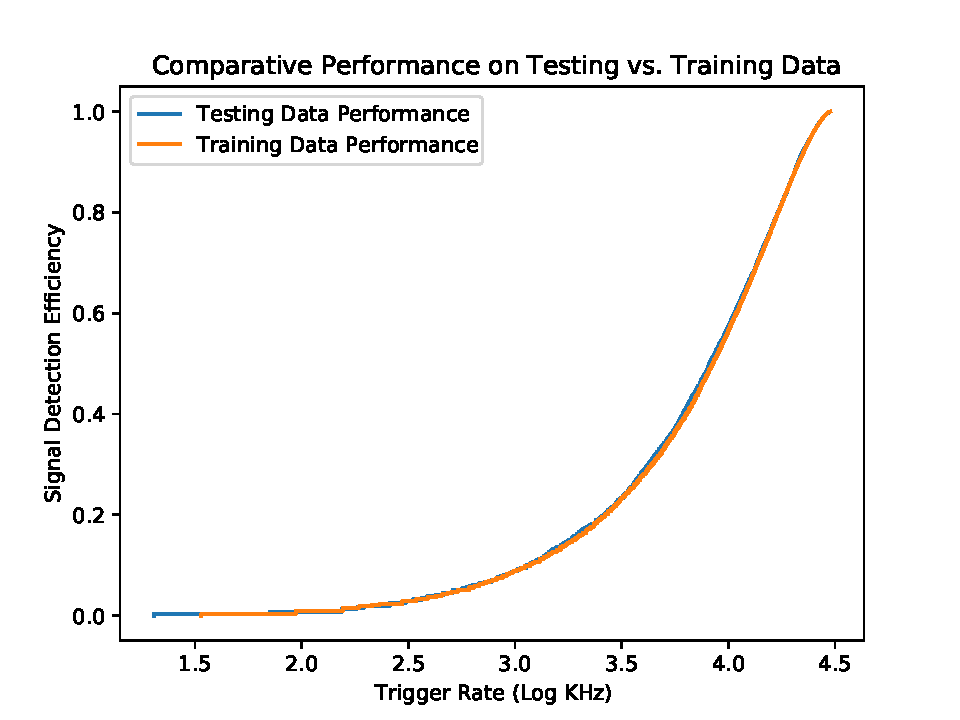
\includegraphics[width=0.9\textwidth]{1trackOvertrainRoc.pdf}

\textbf{2-Track Trigger}\\
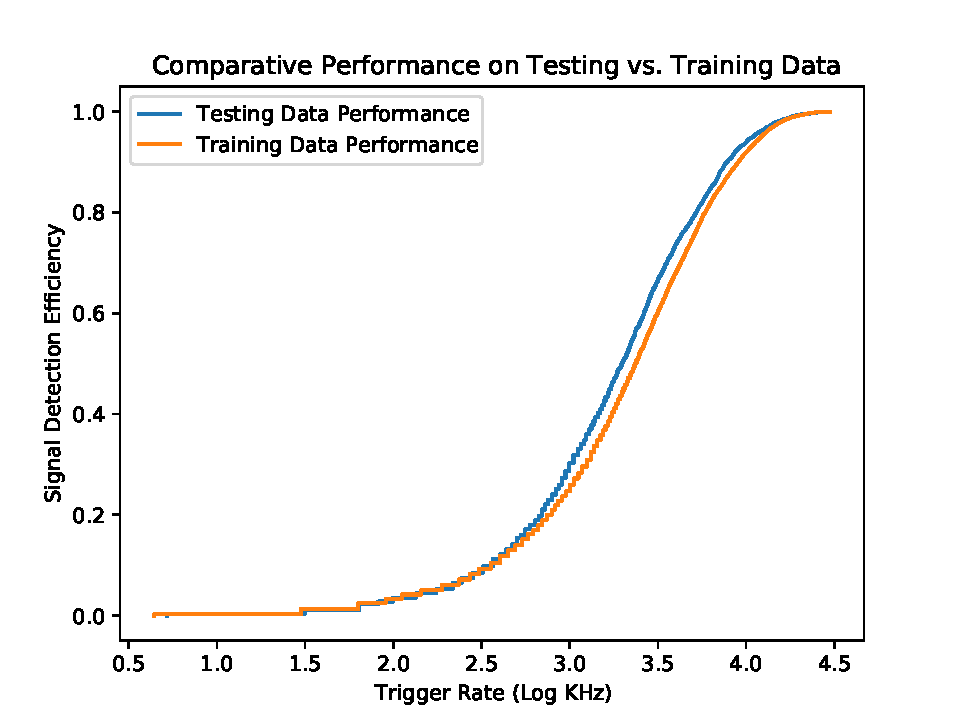
\includegraphics[width=0.9\textwidth]{2trackOvertrainRoc.pdf}
\caption{The performance of the triggers on training vs testing data. No significant performance differences between the two datasets is evidence that no significant overtraining is occurring.}
\label{fig:overtrainRoc}
\end{figure}

\end{document}